\chapter{RESULTADOS E DISCUSS\~AO}
\label{cap:capitulo4}

\section{Desempenho dos modelos}
%Apresentar e comparar os resultados dos diferentes modelos utilizados.

Os resultados obtidos pelos modelos apresentaram variações significativas em termos de precisão, tanto nas previsões pontuais quanto nos intervalos de confiança, refletindo diferentes graus de precisão para cada cenário analisado. A análise dos resíduos revelou-se particularmente interessante, pois evidenciou comportamentos distintos em função da sazonalidade, com variações marcantes observadas em diferentes períodos do ano.

\subsection{Rio Jequitinhonha}

Iniciando pela menor bacia hidrográfica estudada, os resultados revelaram-se bastante satisfatórios, especialmente no que se refere ao modelo de Regressão Linear, que se destacou com previsões precisas, tanto em termos pontuais quanto nos intervalos de confiança. Este modelo demonstrou uma capacidade robusta de capturar a dinâmica hidrológica do rio, refletindo precisão nas métricas e desempenho consistente, aliado a um tempo de execução significativamente reduzido. Em contrapartida, o modelo (simples) SeasonalNaive apresentou resultados abaixo das expectativas em todas as situações avaliadas. (figura \ref{fig:jequiti_SN_WFV})

Com a MAPE extremamente elevada, de 150\%, os resultados indicaram um viés significativo de superestimação, conforme evidenciado pela métrica PBIAS. Verificando a KGE, ficou negativa. Em outras palavras, isso significa que o modelo não apenas falha em capturar a variabilidade dos dados observados, mas também introduz erros que o tornam menos eficaz do que uma abordagem simplista, como utiilizar a média histórica. Embora a análise superficial da qualidade dos intervalos de confiança pudesse sugerir um desempenho satisfatório do modelo, uma inspeção mais detalhada revela uma incongruência: os valores inferiores do intervalo (lo-95) foram calculados abaixo de zero, o que não faz sentido para o rio em questão, pois implicaria na ausência total de vazão, algo inviável para as condições medidas pela estação. Além disso, o atraso (\textit{delay}) da série prevista foi considerável, atingindo 56,88 dias, com um desvio-padrão de 61,3 dias, sugerindo que um evento pode demorar mais de 60 dias para ser refletido na previsão do modelo.

Considerando o desempenho insatisfatório do modelo SN, a análise foi encerrada neste ponto, sem proceder com a avaliação dos resíduos ou a análise da importância das variáveis. O modelo foi incluído apenas para fins comparativos. A análise mais aprofundada será dedicada aos modelos mais complexos, que apresentaram desempenho superior.

\begin{figure}[!h]
	\centering
	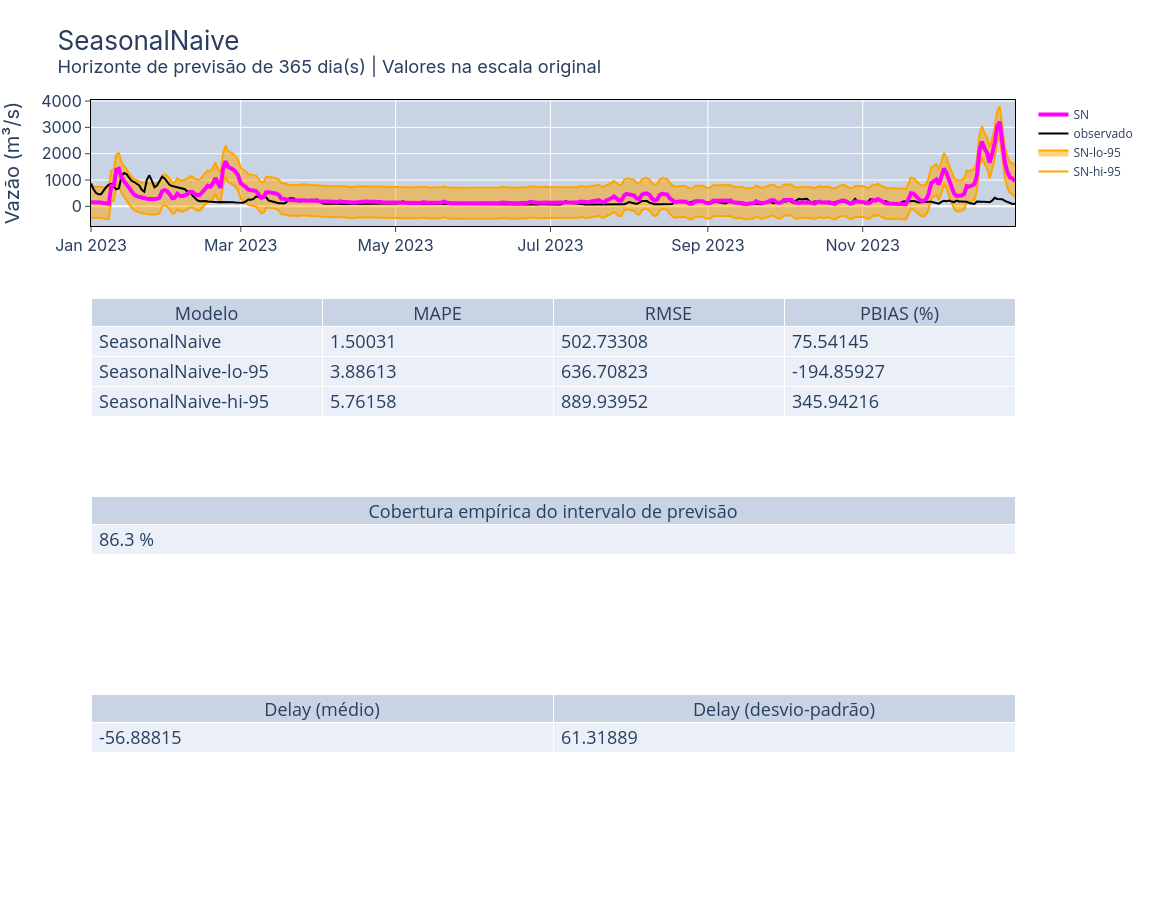
\includegraphics[scale=0.33]{Figuras/jequiti/resultados/SN_WFV.png}
	\caption{Resultado do SeasonalNaive no teste \textit{Walk-Forward Validation}\\(fonte: o autor)}
	\label{fig:jequiti_SN_WFV}
\end{figure}

%\begin{table}[!h]
%	\centering \small
%	\caption{Resultados SeasonalNaive - rio Jequitinhonha \\(fonte: o autor)}
%	\begin{tabular}{|l|r|r|r|r|r|r|} \hline 
	%		\textbf{Horizonte} & \textbf{MAPE} & \textbf{RMSE} & \textbf{PBIAS} \\\hline
	%		1 dia              & 0,871         & 831,44        & -87,11 \\\hline
	%		3 dias             & 1,528         & 1872,25       & 102,71 \\\hline
	%		7 dias             & 1,046         & 1529,13       & 49,64  \\\hline
	%		15 dias            & 0,791         & 1468,02       & -13,46 \\\hline
	%	\end{tabular}
%	\label{tab:sn_jequitinhonha_resultados}
%\end{table}

Os resultados obtidos utilizando o modelo de Regressão Linear mostraram-se bastante promissores.(figura \ref{fig:jequiti_LR_WFV_LOG}) Nesta primeira avaliação, os dados foram log-transformados. Isso é verificável no título, com o uso de ``destransformados''. Os dados foram log-transformados e retornados para a escala original para desenhar o gráfico e ficarem acessíveis para quem lê. \underline{Essa dinâmica no título se manterá por todo trabalho}.

Partindo pela KGE calculada, o resultado mostrou-se excelente. Recordando: quanto mais próxima de 1, melhor. Este valor sugere que o modelo é eficaz na previsão do comportamento hidrológico do sistema em análise, oferecendo previsões que estão bem alinhadas com os dados observados. A MAPE de 14\% sugere que o modelo tem uma precisão razoável e é bastante confiável. O modelo apresentou um viés sistemático de subestimar os resultados, conforme aponta a PBIAS de -1,76\%. Considerando todas as métricas, o resultado indica que o modelo teve um desempenho global muito bom. A KGE alta é particularmente indicativa de um bom ajuste global, com o modelo capturando bem tanto a dinâmica quanto a magnitude dos dados observados.

Considerando a qualidade dos intervalos de previsão, a cobertura observada de 97,81\% excedeu o intervalo teórico calculado de 95\%, o que, à primeira vista, poderia ser interpretado como um desempenho satisfatório. No entanto, o limite superior do intervalo (hi-95) mostrou-se excessivamente elevado nos meses de janeiro e fevereiro, o que pode comprometer a interpretação dos resultados. Isso ocorre porque intervalos de previsão excessivamente amplos podem capturar praticamente qualquer valor observado, reduzindo a utilidade prática da previsão.

É importante destacar que os intervalos de previsão são calculados a partir dos erros do modelo durante a etapa de treinamento (\textit{in-sample residuals}). Para uma análise mais aprofundada desse comportamento, é necessário examinar os dados anteriores a 2023. A figura \ref{fig:jequiti_LR_final_2022_detalhe} revela que, nos últimos dias de 2022, houve observações significativamente elevadas. É provável que os erros associados a esse período mais próximo tenham influenciado a amplitude dos intervalos de previsão subsequentes. Essa interpretação é suportada pela observação de que o comportamento ao final de 2023 foi mais estável, possivelmente devido à ausência de eventos ruidosos imediatamente anteriores (meses de maio a agosto).

\begin{figure}[!h]
	\centering
	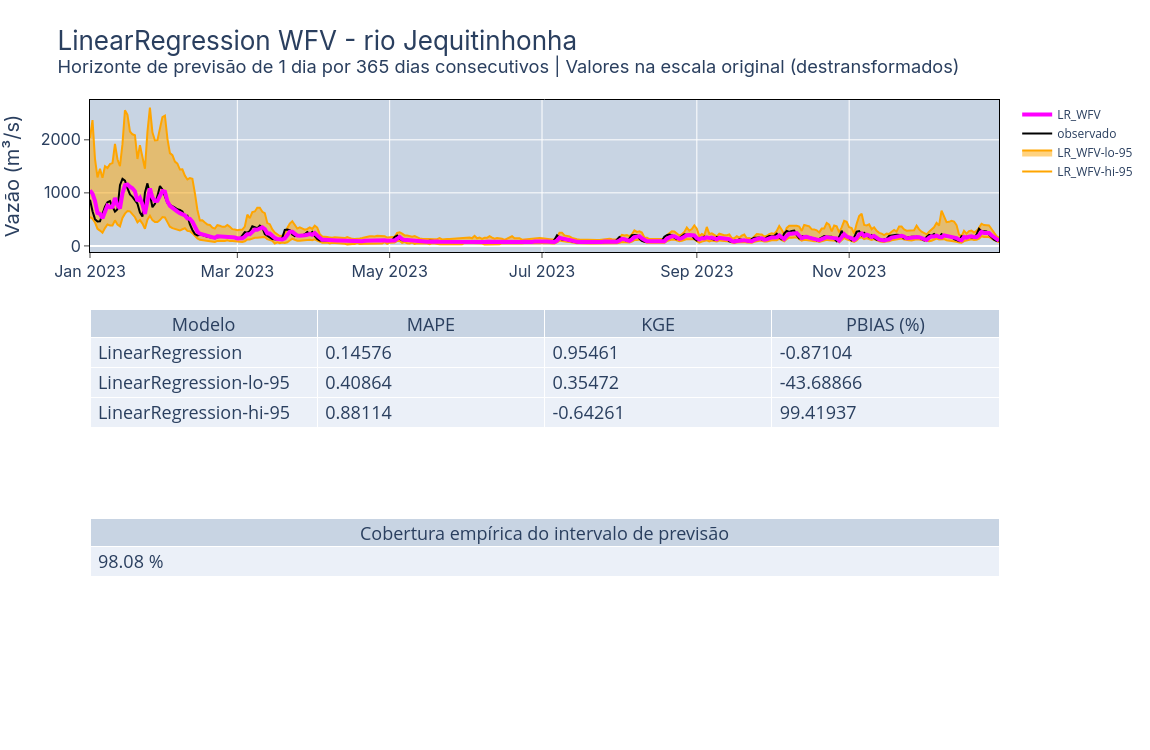
\includegraphics[scale=0.33]{Figuras/jequiti/resultados/LR_WFV_LOG.png}
	\caption{\textit{Walk-Forward Validation} para o modelo Regressão Linear - LR\\(fonte: o autor)}
	\label{fig:jequiti_LR_WFV_LOG}
\end{figure}

\begin{figure}[!h]
	\centering
	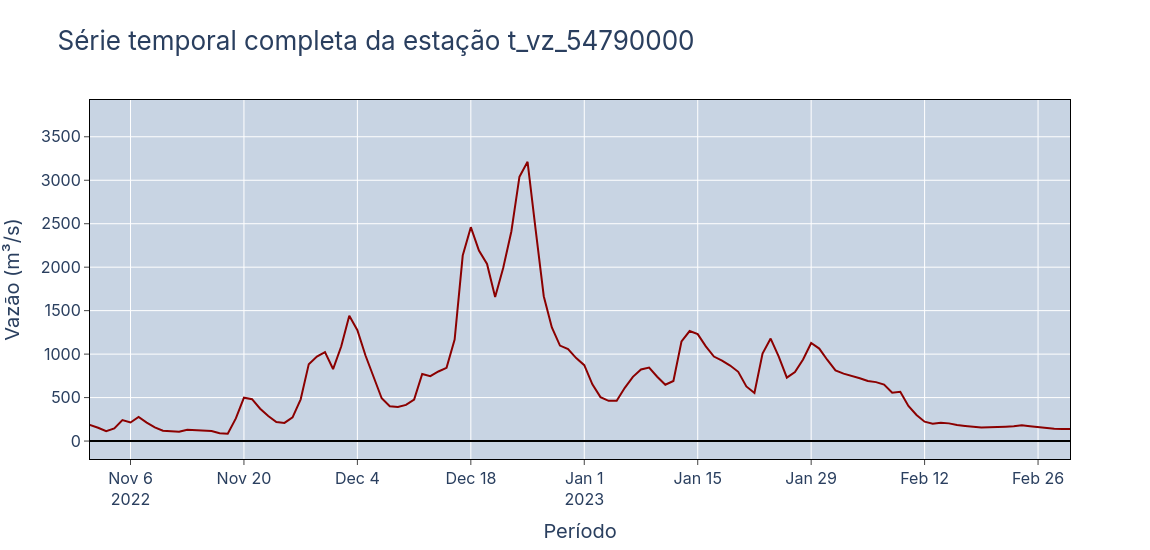
\includegraphics[scale=0.33]{Figuras/jequiti/resultados/LR_final_2022_detalhe.png}
	\caption{Detalhe do trecho final dos dados, em 2022, usados para treinamento.\\(fonte: o autor)}
	\label{fig:jequiti_LR_final_2022_detalhe}
\end{figure}

A análise de \textit{delay} mostrou um resultado médio de $-0,87$. Se pegar a série prevista pelo modelo e comprimir linearmente em $-0,87$, ambas as sequências serão idênticas, ou seja, a série prevista será a série observada. Considerando que os dados estão numa frequência diária, isso pode ser interpretado como o modelo atrasando a previsão em $0,87$ dias, o que seria menos de 24 horas entre o evento ocorrer e ele ser percebido na previsão. Afirmar que o modelo está atrasado 20,88 horas, talvez, não convirja com a realidade, por isso que se considerar o desvio-padrão no resultado, confere mais coerência, pois indicaria que o atraso percebido no fenômeno é de cerca de um dia e meio, dois dias.

\begin{figure}[!h]
	\centering
	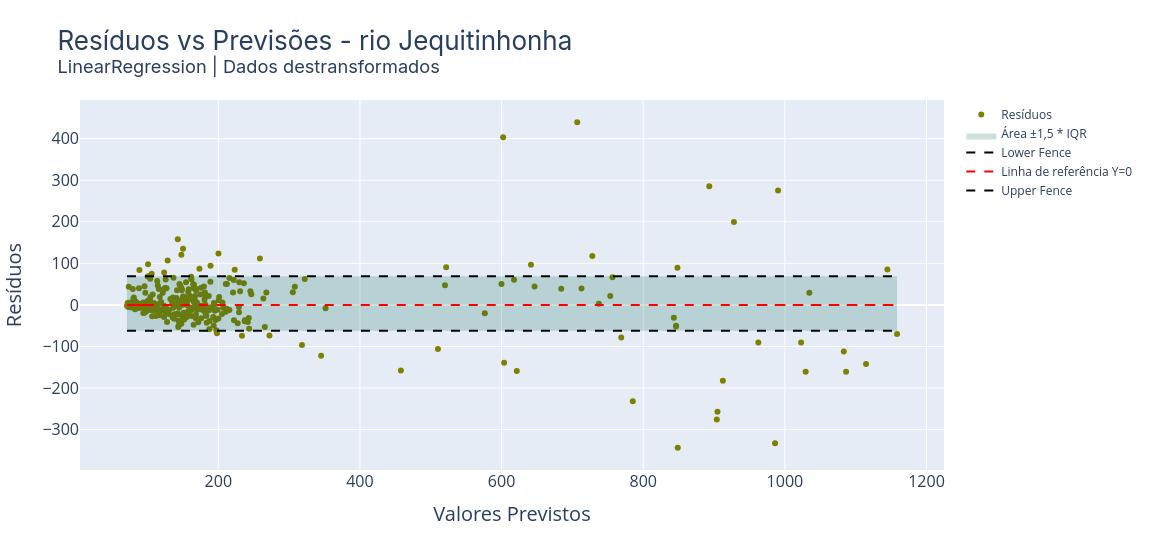
\includegraphics[scale=0.33]{Figuras/jequiti/resultados/LR_WFV_LOG_RESID_x_PREV.png}
	\caption{Resíduos da previsão versus os valores das previsões.\\(fonte: o autor)}
	\label{fig:jequiti_LR_WFV_LOG_RESID_x_PREV}
\end{figure}

Na figura \ref{fig:jequiti_LR_WFV_LOG_RESID_x_PREV} podemos observar a concentração dos resíduos em torno de zero. A linha vermelha tracejada é onde o valor previsto e observado são iguais, designando a previsão perfeita, com resíduo $0$. Este é o comportamento que se espera, idealmente, os resíduos estarem distribuídos aleatoriamente em torno de zero, sem padrões evidentes (nenhuma tendência clara de curvatura ou cone). Contudo, à medida que se caminha sobre a linha vermelha tracejada, aumentando o valor no eixo x, há um aumento na dispersão dos resíduos. A área sombreada demarcada são os valores calculados para \textit{lower fence} e \textit{upper fence} a partir do primeiro ($-14,68$) e terceiro ($19,93$) quartil, que aqui resultaram em $-66,60$ e $71,85$, respectivamente. Entre estes valores é onde se espera que os resíduos estejam distribuídos (houve uma prevalência de $87,95\%$ dos resíduos nesta área), o que fica de fora dessas faixas pode ser interpretado como um \textit{outlier}. Considerando que os dados de treinamento não foram tratados para valores \textit{outliers}, isso parece estar se refletindo neste resultado, mesmo com a transformação logarítmica. O modelo não captou corretamente os valores elevados nos dados observados, por isso resíduos tão grandes assim, ainda que tenha apresentado um comportamento geral bom, como visto nas métricas anteriormente. Outro fator a se considerar também é que por estar na escala log, qualquer pequena variação nesta escala, quando retornada para a escala original, pode significar números elevados.

Veja na figura \ref{fig:jequiti_LR_WFV_LOG_RESID_x_TEMPO} como os resíduos estão dispersos ao longo do tempo. No início do ano e final do ano, exatamente quando os eventos de chuva mais ocorrem, o modelo tende a se dispersar. No início do ano, como discutido anteriormente, pode ser que devido às vazões elevadas do final do ano de 2022, isso tenha causado ruídos em excesso na previsão do modelo. Quando houve vazões mais moderadas, os resíduos foram também mais moderados, como pode-se observar no final do ano de 2023, em que a influência imediata é o meio do ano, meses de inverno, e início de primavera. Quando da estação de baixa dos rios, os meses de outono e inverno, os resíduos estiveram bem alinhados em torno do $0$. Para encerrar essa análise, a figura \ref{fig:jequiti_LR_WFV_LOG_RESID_x_CURVA_NORMAL} apresenta que os resíduos estão próximos da normalidade quanto à distribuição destes em torno de $0$, com uma assimetria de $1,46$, o que pode ser considerada baixa, mas não descartável. O valor positivo para assimetria sugere que houve casos em que o modelo subestimou os valores (existe uma cauda à direita do centro dos dados), o que combina com os gráficos anteriores de dispersão. Mas cabe destacar que os resíduos não estão significativamente desviados em nenhuma direção, apresentam distribuição aleatória e não sistemática e este é um comportamento desejado. A análise da função de autocorrelação (ACF) está na figura \ref{fig:jequiti_LR_WFV_LOG_RESID_ACF} e aqui é analisado se existe independência ou dependência temporal entre os resíduos. A área sombreada representa a faixa ideal de permanência dos resíduos, onde se espera que a maioria dos resíduos esteja concentrada caso não haja autocorrelação significativa. Algumas \textit{lags} estão fora destes limites (picos), mais precisamente, \textit{lags} que estão mais próximas da \textit{lag} de referência. Este comportamento indica que o modelo pode ser refinado para melhor capturar dinâmicas temporais, possivelmente incorporando termos de tendência. Mas no aspecto geral, está bom o comportamento dos resíduos. Para melhorar os resíduos com valores tão elevados um tratamento de \textit{outliers} pode verter bons resultados.

\begin{figure}[!h]
	\centering
	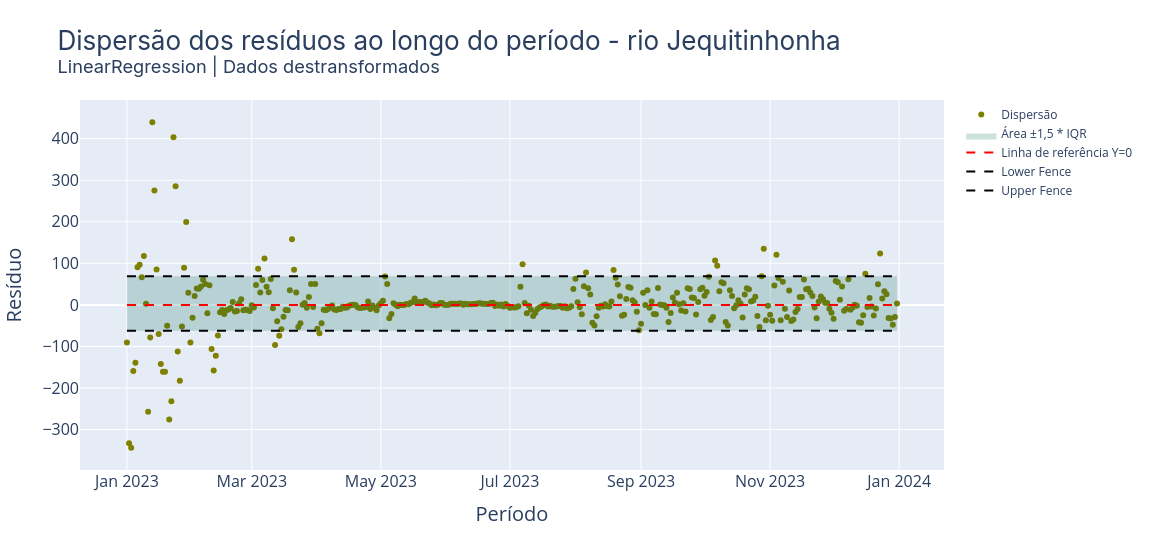
\includegraphics[scale=0.33]{Figuras/jequiti/resultados/LR_WFV_LOG_RESID_x_TEMPO.png}
	\caption{Resíduos da previsão ao longo do tempo.\\(fonte: o autor)}
	\label{fig:jequiti_LR_WFV_LOG_RESID_x_TEMPO}
\end{figure}

\begin{figure}[!h]
	\centering
	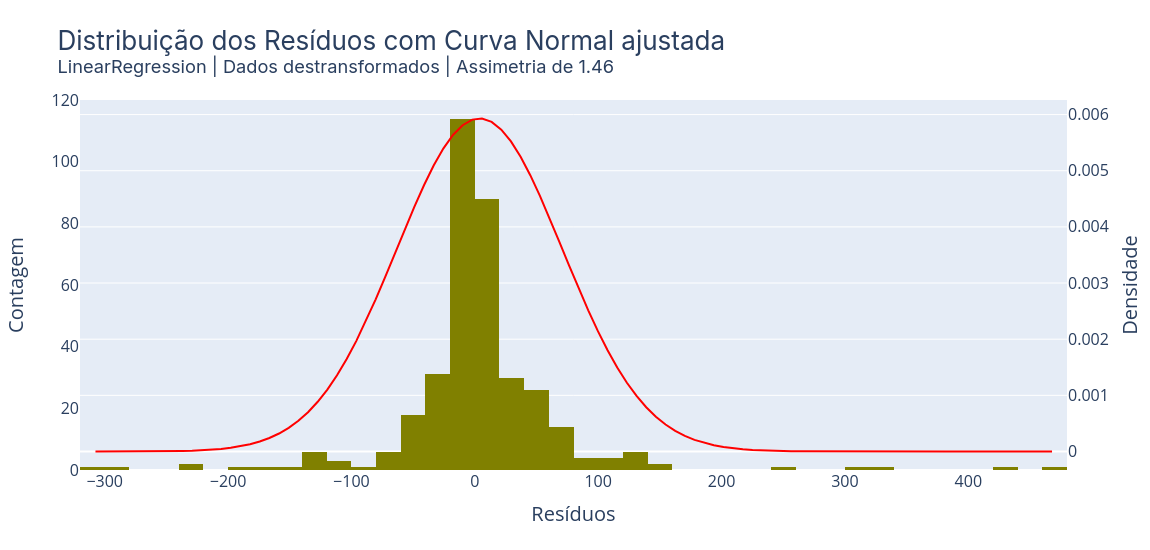
\includegraphics[scale=0.33]{Figuras/jequiti/resultados/LR_WFV_LOG_RESID_x_CURVA_NORMAL.png}
	\caption{Histograma dos resíduos.\\(fonte: o autor)}
	\label{fig:jequiti_LR_WFV_LOG_RESID_x_CURVA_NORMAL}
\end{figure}

\begin{figure}[!h]
	\centering
	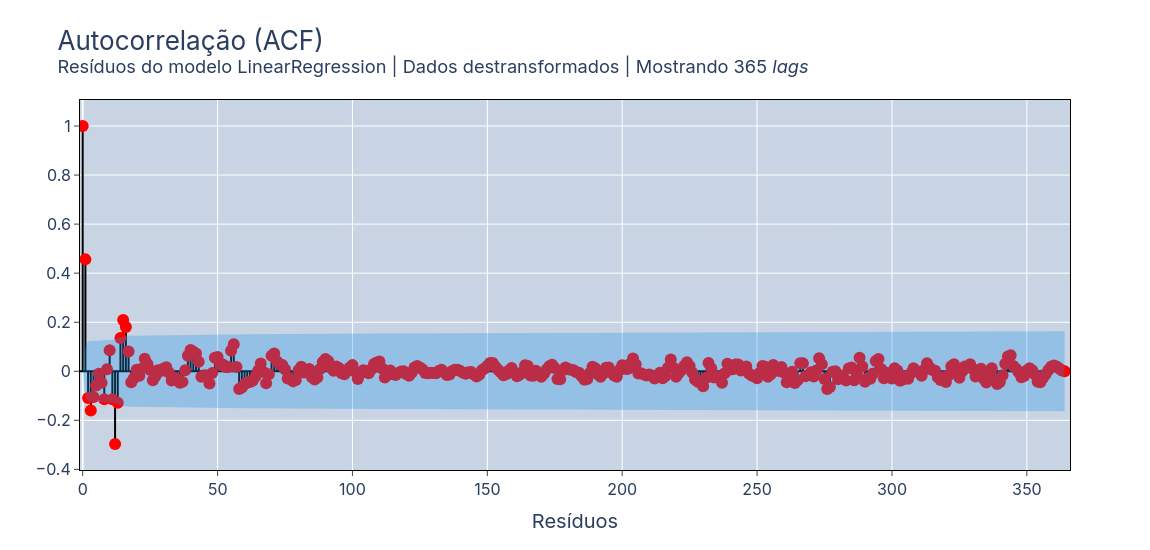
\includegraphics[scale=0.33]{Figuras/jequiti/resultados/LR_WFV_LOG_RESID_ACF.png}
	\caption{Resíduos da previsão ao longo do tempo.\\(fonte: o autor)}
	\label{fig:jequiti_LR_WFV_LOG_RESID_ACF}
\end{figure}
\clearpage

Agora os resultados sem emprego da log-transformação, com os dados originais. Salientando que para o modelo LR não é correto aplicar os dados originais na escala em que se encontram, foi precisar realizar normalização antes empregando algoritmo MinMax. Este algoritmo coloca todos os dados em valores entre $0$ e $1$, sendo o valor mínimo correspondente a cada série temporal passado para $0$ e o valor máximo é passado para $1$. Com os demais valores é feito, basicamente, uma regra de três para achar o valor correspondente na escala entre $0$ e $1$.

Dito isso, o resultado para os dados originais ficou levemente inferior ao modelo com os dados log-transformados. Em todas as métricas que se avaliar o resultado ficou piorado. Um comportamento destacado foi as faixas nos valores dos intervalos de previsão. Diferentemente do comportamento anterior (figura \ref{fig:jequiti_LR_WFV_LOG}), em que houve uma prevalência de faixas elevadas no início do ano, neste resultado o início do ano esteve, digamos, bem comportado. Ao decorrer do ano que os intervalos incrementaram, ali a partir do mês de fevereiro, e foram aumentando até o fim do ano. Isso pode ser um indicativo de que o modelo teve problemas na estabilidade de longo prazo, acumulando incertezas no período.

Ainda que tenha apresentado uma KGE inferior, bem como nas demais métricas, quando se observa o comportamento dos resíduos, houve uma prevalência de $90,96\%$ dos resíduos na área sombreada no gráfico de dispersão.(figura \ref{fig:jequiti_LR_WFV_SCLD_RESID_x_PREV}) Isso significa que houve menos \textit{outliers} nas previsões. Pode-se verificar também este resultado na figura \ref{fig:jequiti_LR_WFV_SCLD_RESID_x_TEMPO}, no início do ano, em que menos \textit{outliers} estão presentes, ainda que na porção final do ano tenha aparecido alguns a mais que não foram vistos na análise anterior (figura \ref{fig:jequiti_LR_WFV_LOG_RESID_x_TEMPO}). Para os dados originais, ainda que nas métricas pareça piorado, pela análise dos resíduos o modelo mostrou boa estabilidade nas previsões pontuais. Quando se considera os intervalos de previsão, precisa considerar com parcimônia, visto que o crescimento dos valores superioes (hi-95) e valores de vazão $0 m^3/s$ na faixa inferior (lo-95) indicam instabilidade de longo prazo.

Para a análise de \textit{delay}, o mesmo feito anteriormente serve para este: aplicar o valor do desvio-padrão parece ser mais coerente com o comportamento real, sendo que aqui houve uma piora significativa no atraso, passando para mais de 3 dias ($3,78$).

Caminhando para o fim, o histograma e curva-normal apresentou uma assimetria consideravelmente superior ($3,38$) ao resultado de antes, com presença de cauda longa à direita. O modelo teve tendência de subestimar os resultados, o que é verificável pelo PBIAS. Na figura \ref{fig:jequiti_LR_WFV_SCLD_RESID_ACF} é possível perceber picos fora do intervalo de confiança. Depois de cerca de 10 lags, os pontos de autocorrelação ficam dentro desta faixa, indicando que a maioria dos resíduos após esse ponto não está significativamente correlacionada com valores anteriores. Este pontos vermelhos no início do gráfico indicam que pode haver correlações significativas entre os resíduos com pequenos \textit{lags}, o que sugere, nos primeiros períodos, que os resíduos estão correlacionados com os valores anteriores. Isso é indicativo de que o modelo pode não estar capturando totalmente a estrutura temporal dos dados. Pode ser necessário ajustar o modelo, adicionar variáveis que expliquem essa dependência temporal, ainda que variáveis de valor acumulado tenham sido inseridas exatamente na intenção de capturar tais comportamentos. Mas claramente precisaria aprimorar.

\begin{figure}[!h]
\centering
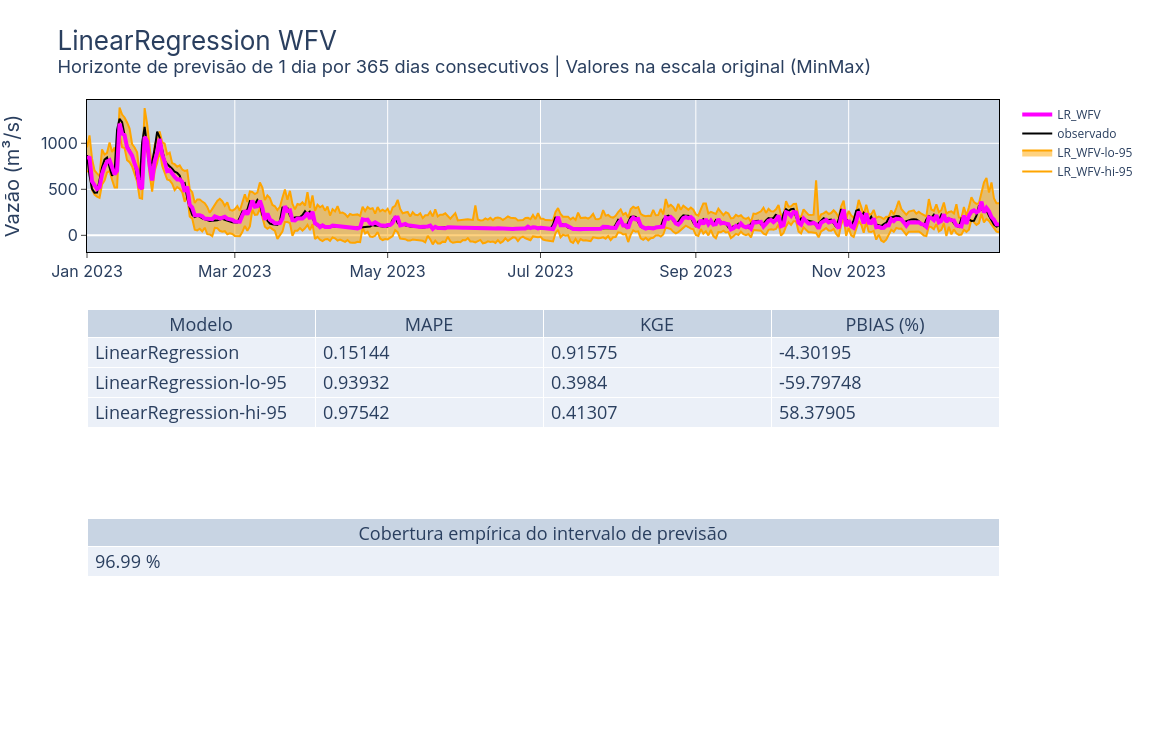
\includegraphics[scale=0.33]{Figuras/jequiti/resultados/LR_WFV_SCLD.png}
\caption{\textit{Walk-Forward Validation} para o modelo Regressão Linear - LR.\\(fonte: o autor)}
\label{fig:jequiti_LR_WFV_SCLD}
\end{figure}

\begin{figure}[!h]
\centering
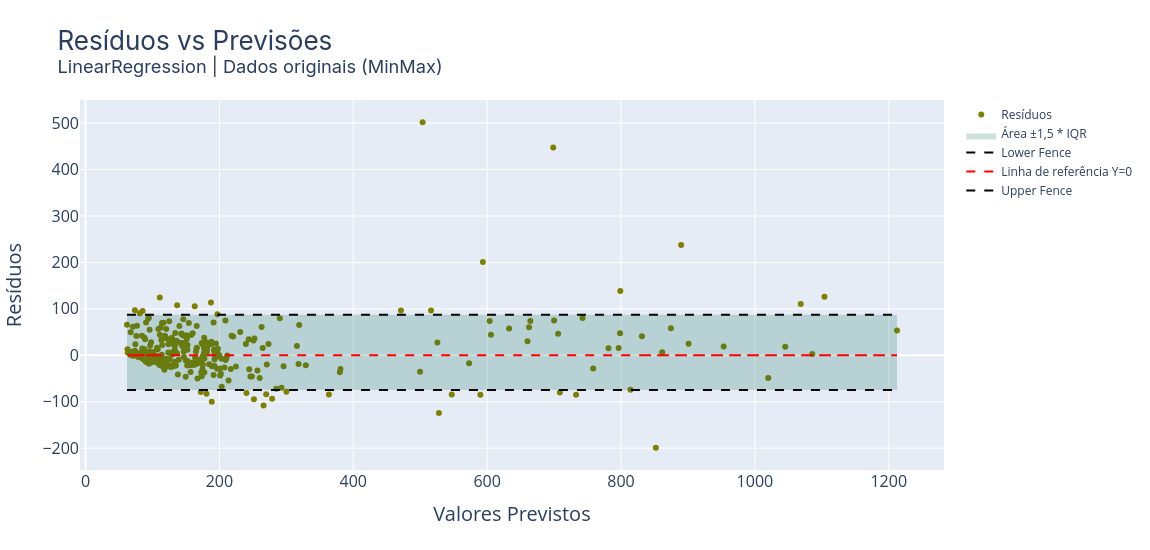
\includegraphics[scale=0.33]{Figuras/jequiti/resultados/LR_WFV_SCLD_RESID_x_PREV.png}
\caption{Dispersão dos resíduos.\\(fonte: o autor)}
\label{fig:jequiti_LR_WFV_SCLD_RESID_x_PREV}
\end{figure}

\begin{figure}[!h]
\centering
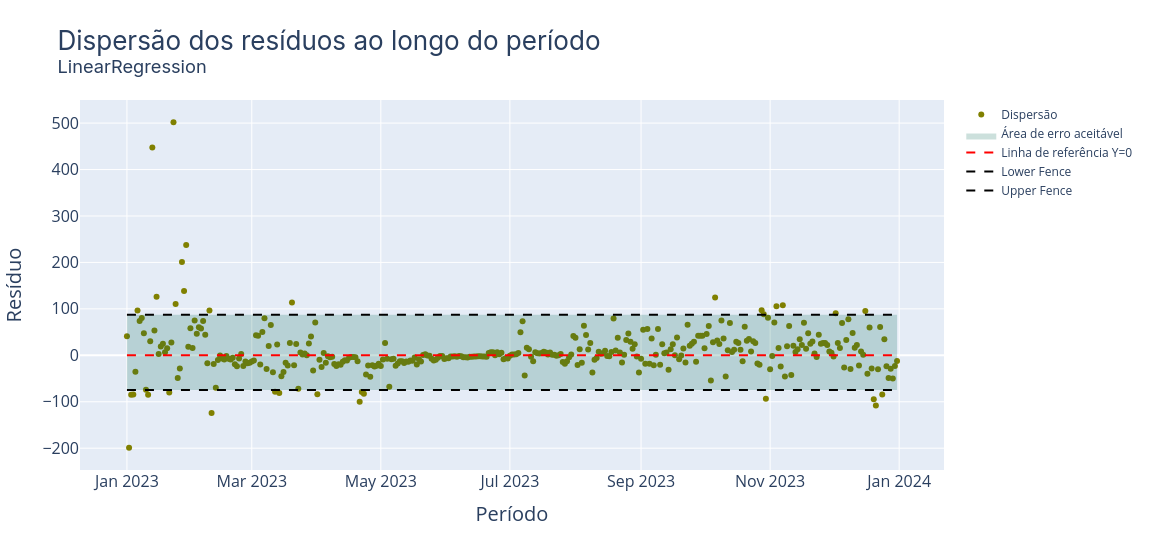
\includegraphics[scale=0.33]{Figuras/jequiti/resultados/LR_WFV_SCLD_RESID_x_TEMPO.png}
\caption{Dispersão dos resíduos ao longo do ano.\\(fonte: o autor)}
\label{fig:jequiti_LR_WFV_SCLD_RESID_x_TEMPO}
\end{figure}

\begin{figure}[!h]
\centering
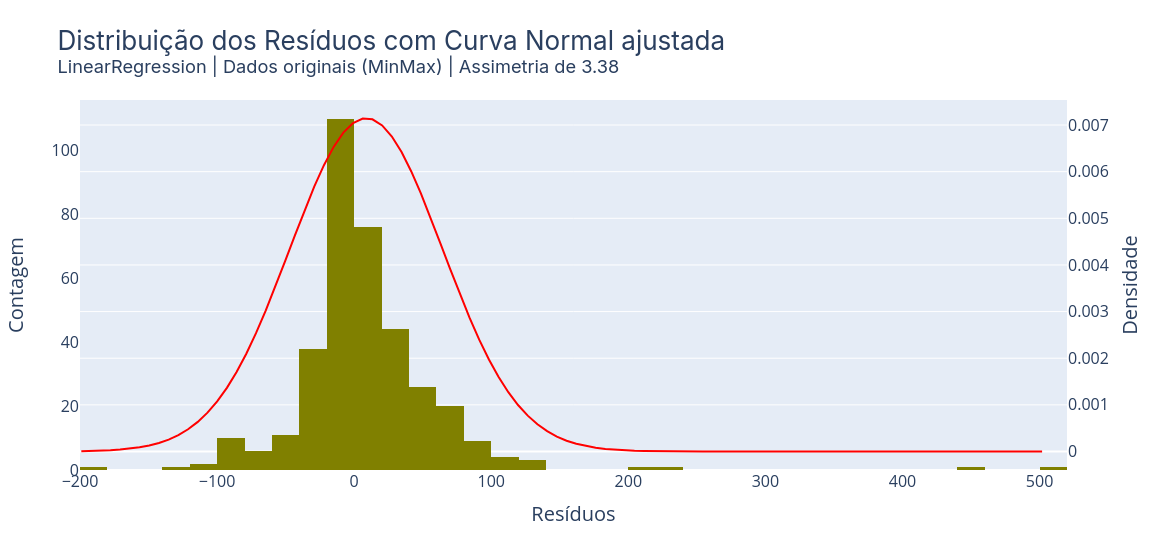
\includegraphics[scale=0.33]{Figuras/jequiti/resultados/LR_WFV_SCLD_RESID_x_CURVA_NORMAL.png}
\caption{Histograma e curva-normal dos resíduos.\\(fonte: o autor)}
\label{fig:jequiti_LR_WFV_SCLD_RESID_x_CURVA_NORMAL}
\end{figure}

\begin{figure}[!h]
\centering
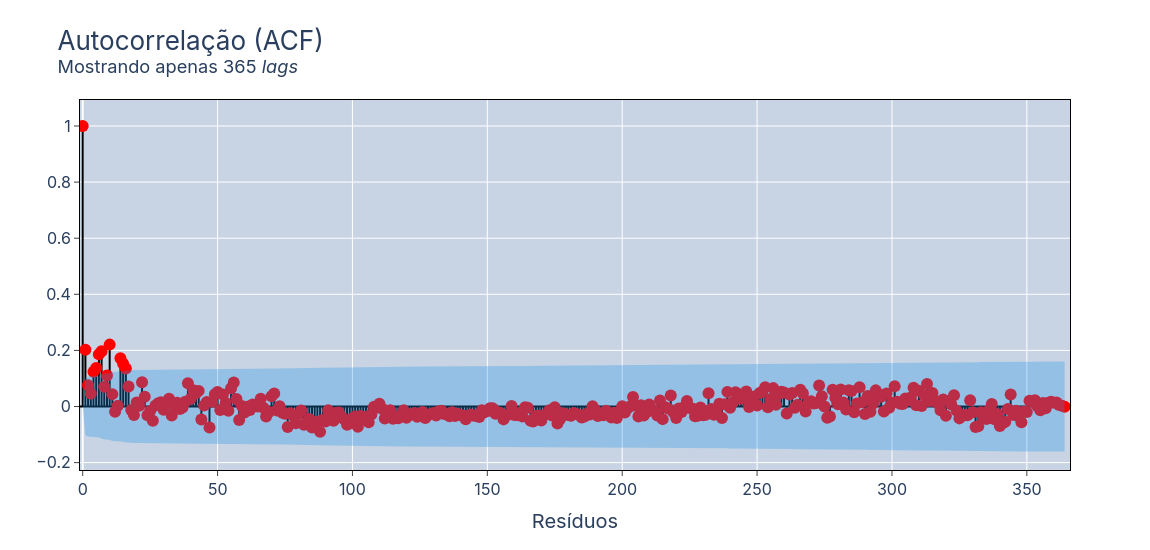
\includegraphics[scale=0.33]{Figuras/jequiti/resultados/LR_WFV_SCLD_RESID_ACF.png}
\caption{Gráfico ACF dos resíduos.\\(fonte: o autor)}
\label{fig:jequiti_LR_WFV_SCLD_RESID_ACF}
\end{figure}
\clearpage

Passando agora à análise dos modelos principais deste trabalho, cujos resultados serão comparados ao modelo de referência, optou-se por realizar a análise de forma concomitante, uma vez que ambos os modelos apresentaram comportamentos similares, embora o modelo RandomForest tenha demonstrado um desempenho superior ao CatBoost.

Na métrica KGE, comparando-se os resultados com o comportamento ilustrado na figura \ref{fig:jequiti_LR_WFV_LOG}, observa-se que ambos os modelos não conseguiram superar o modelo de referência, com destaque para o CB, que apresentou uma performance consideravelmente inferior. No entanto, ao considerar a precisão percentual média, avaliada pela métrica MAPE, ambos os modelos baseados em árvores apresentaram melhorias em relação ao modelo de referência, evidenciando um desempenho superior em termos de erro percentual médio.

A KGE, relembrando, combina três aspectos fundamentais: variabilidade, viés e correlação entre os dados observados e previstos. Considerando esses fatores, com os dados log-transformados, o modelo LR capturou de forma mais eficaz os três aspectos mencionados. É provável que a linearização tenha sido um fator determinante para o bom desempenho deste modelo olhando por esta métrica, uma vez que, ao analisar a MAPE, os modelos não-lineares (CB e RF) apresentaram desempenhos melhores. Um desempenho médio percentual melhor pode dever-se à resiliência dos modelos não-lineares à sua robustez diante de valores discrepantes, aos quais o modelo linear é mais sensível.

Observa-se que tanto o CB quanto o RF apresentaram intervalos de previsão menos amplos no início do ano, em comparação com o modelo LR, mesmo impactados pelas vazões elevadas no final de 2022 (figura \ref{fig:jequiti_LR_final_2022_detalhe}). Em termos de previsão pontual, ambos os modelos não lineares demonstraram-se robustos. No entanto, ao analisar a cobertura empírica dos intervalos de previsão, o modelo RF mostrou-se consideravelmente defasado em relação aos modelos LR e CB. Isso pode ser explicado pela possível ``otimização'' excessiva do modelo ao calcular os intervalos, ao presumir uma repetição dos eventos e erros passados, resultando em intervalos estreitos. Esse fenômeno é descrito por \citet{RobHyndman_prediction_intervals}. Apesar disso, a cobertura empírica de $80\%$ do modelo RF ainda pode ser considerada satisfatória, e a cobertura de $88\%$ obtida pelo CB demonstra um bom desempenho.

Pode-se inferir que os modelos CB e RF conseguiram equilibrar a previsão pontual, indicada pela MAPE de $0,12$, com os intervalos de previsão. Um ajuste de hiperparâmetros poderia potencialmente melhorar esse desempenho. Em relação ao PBIAS, ambos os modelos apresentaram um desvio sistemático, subestimando os valores previstos. No que diz respeito ao \textit{delay}, todos os modelos, incluindo o LR, apresentaram um comportamento semelhante, com um atraso de aproximadamente 1 a 2 dias para que um evento na série observada fosse captado nas previsões. Essa análise leva em consideração o desvio-padrão.

\begin{figure}[!h]
\centering
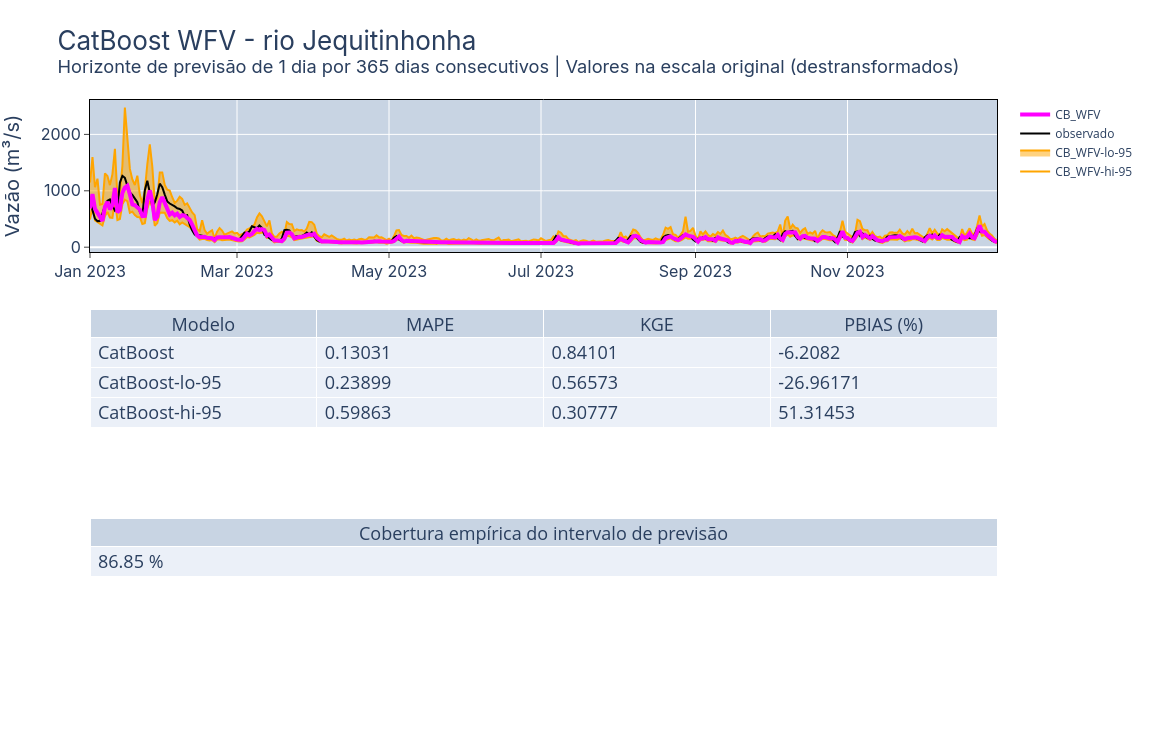
\includegraphics[scale=0.33]{Figuras/jequiti/resultados/CB_WFV_LOG.png}
\caption{\textit{Walk-Forward Validation} para o modelo CatBoost - CB.\\(fonte: o autor)}
\label{fig:jequiti_CB_WFV_LOG}
\end{figure}

\begin{figure}[!h]
\centering
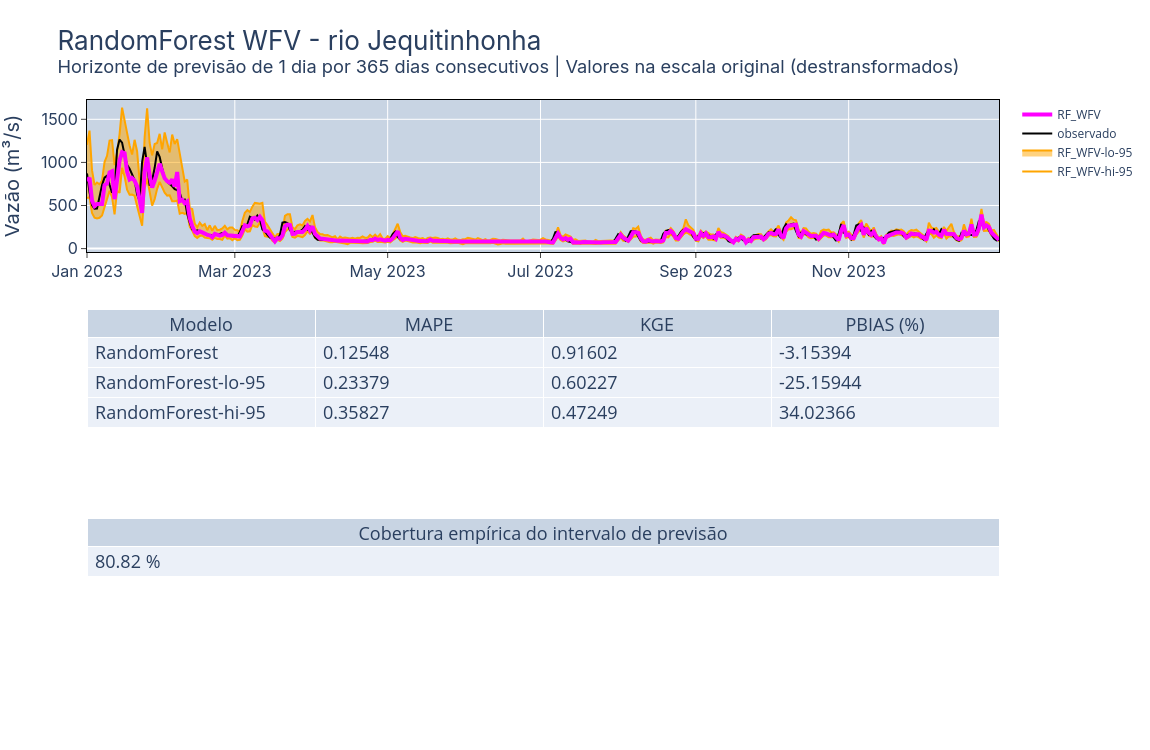
\includegraphics[scale=0.33]{Figuras/jequiti/resultados/RF_WFV_LOG.png}
\caption{\textit{Walk-Forward Validation} para o modelo RandomForest - RF.\\(fonte: o autor)}
\label{fig:jequiti_RF_WFV_LOG}
\end{figure}

Os resíduos em modelos não-lineares podem ser mais difíceis de interpretar porque esses modelos capturam interações e padrões complexos. Porém, mesmo assim, detectar padrões sistemáticos nos resíduos ajuda a elucidar se os modelos conseguiram capturar todas as nuances dos dados.

Em ambos os casos, não houve prevalência de comportamento anormal para os resíduos. Estiveram aleatoriamente distribuídos em torno de $0$, com uma menção importante para a maior dispersão de possíveis valores \textit{outliers} para o modelo CB à medida que as medições aumentaram.(figura \ref{fig:jequiti_CB_WFV_LOG_RESID_x_PREV}).

A dispersão ao longo do tempo foi praticamente a mesma para ambos os modelos, com resíduos de valor elevado mais presentes no início da série. (figuras \ref{fig:jequiti_CB_WFV_LOG_RESID_x_TEMPO} \ref{fig:jequiti_RF_WFV_LOG_RESID_x_TEMPO}) Aqui vale a interpretação usada para o modelo de referência, de que os valores elevados aferidos em final de 2022 possam ter interferido. Houve uma prevalência de $84,11\%$ e $86,03\%$, respectivamente CB e RF, dos resíduos na área sombreada, correspondente à área de erro aceitável.

\begin{figure}[!h]
\centering
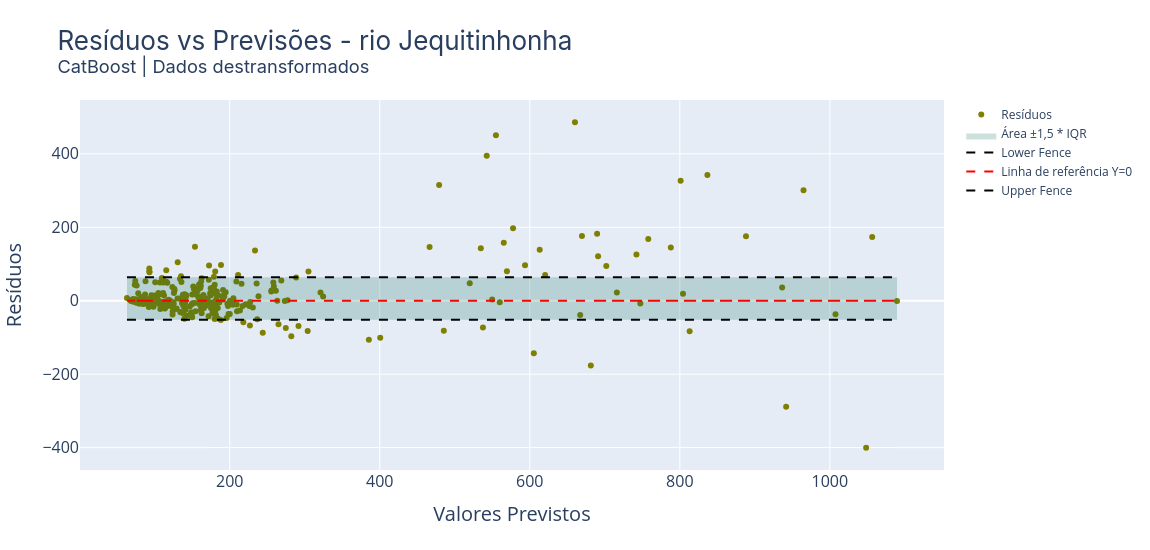
\includegraphics[scale=0.33]{Figuras/jequiti/resultados/CB_WFV_LOG_RESID_x_PREV.png}
\caption{Resíduos da previsão \textit{versus} os valores das previsões.\\(fonte: o autor)}
\label{fig:jequiti_CB_WFV_LOG_RESID_x_PREV}
\end{figure}

\begin{figure}[!h]
\centering
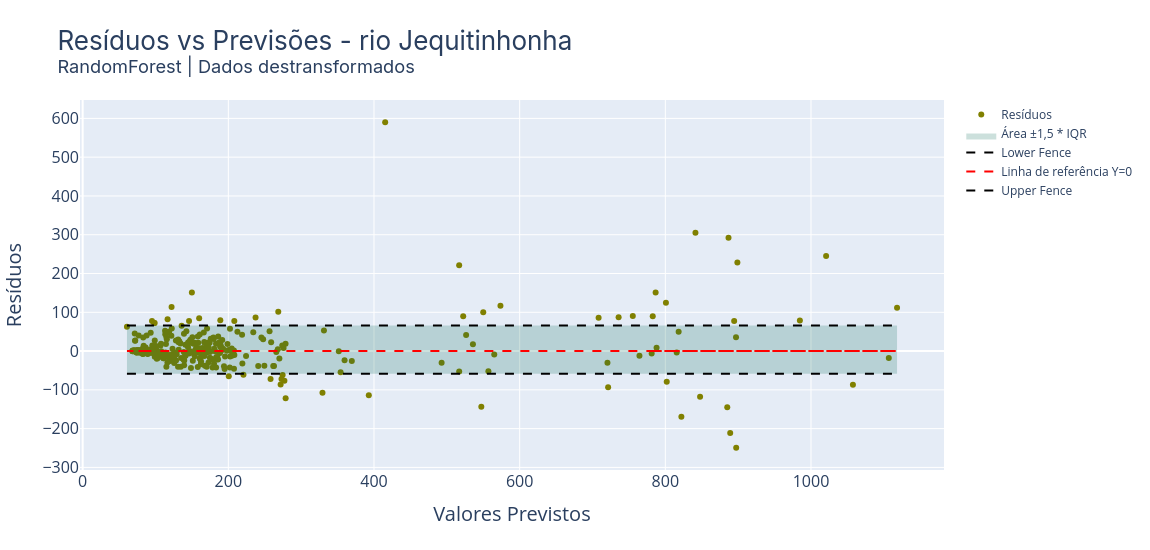
\includegraphics[scale=0.33]{Figuras/jequiti/resultados/RF_WFV_LOG_RESID_x_PREV.png}
\caption{Resíduos da previsão \textit{versus} os valores das previsões.\\(fonte: o autor)}
\label{fig:jequiti_RF_WFV_LOG_RESID_x_PREV}
\end{figure}

\begin{figure}[!h]
\centering
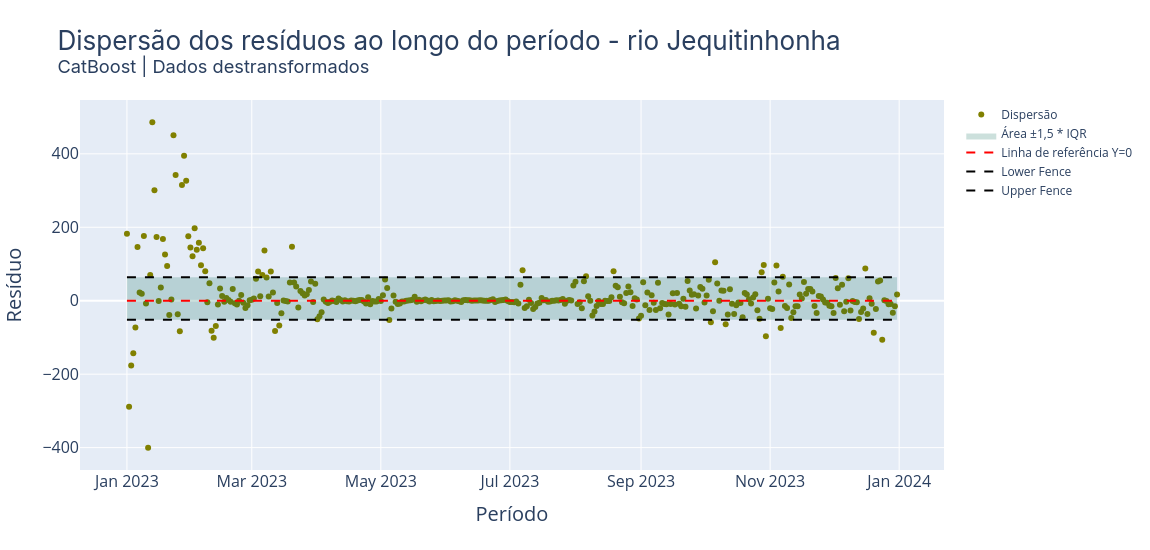
\includegraphics[scale=0.33]{Figuras/jequiti/resultados/CB_WFV_LOG_RESID_x_TEMPO.png}
\caption{Dispersão dos resíduos ao longo do ano.\\(fonte: o autor)}
\label{fig:jequiti_CB_WFV_LOG_RESID_x_TEMPO}
\end{figure}

\begin{figure}[!h]
\centering
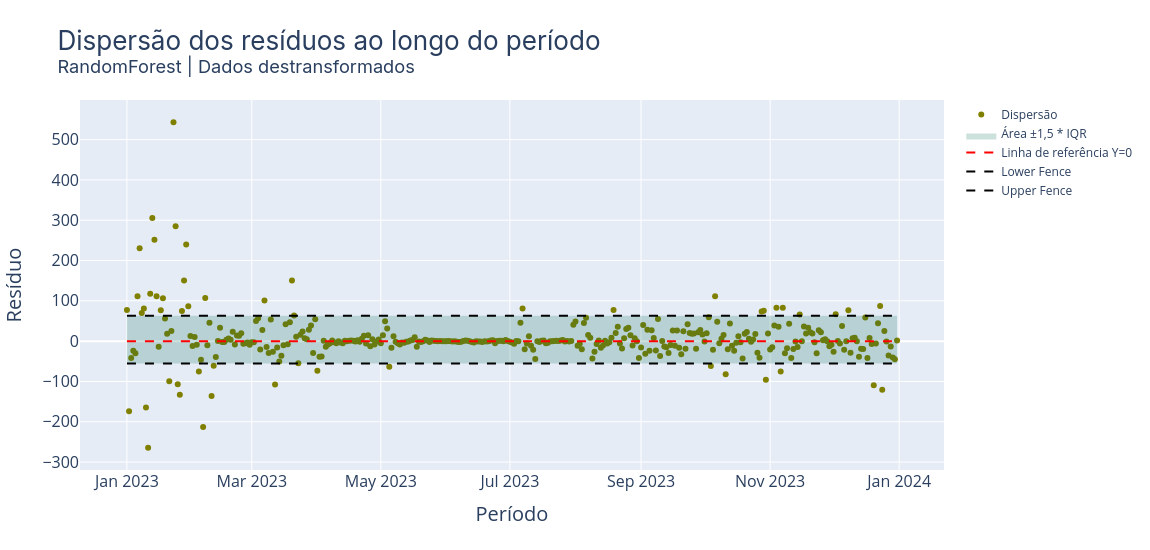
\includegraphics[scale=0.33]{Figuras/jequiti/resultados/RF_WFV_LOG_RESID_x_TEMPO.png}
\caption{Dispersão dos resíduos ao longo do ano.\\(fonte: o autor)}
\label{fig:jequiti_RF_WFV_LOG_RESID_x_TEMPO}
\end{figure}
\clearpage

\section{Importância das variáveis}
%Analisar a importância das variáveis contínuas e categóricas na previsão (feature importance).

\section{Discuss\~ao dos resultados}
%Interpretar os resultados e discutir as limitações. Se possível, comparar com estudos anteriores.